\begin{figure}[h]
	\centering
	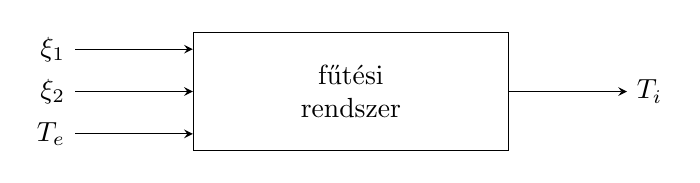
\begin{tikzpicture}[>=stealth,
	outer/.style={draw=gray,dashed,thick,inner sep=5pt}]
	
	% nagy blokkok
	\node[draw,rectangle, minimum height=1.5cm,minimum width=4cm] (plant) at (0,2.5) {\parbox{2cm}{\centering fűtési rendszer}};
	%\node[draw,rectangle, minimum height=1.5cm,minimum width=3cm] (Control) at (0,2.5) {\parbox{2.5cm}{\centering modellalapú\\szabályzó}};
	
	% szaggatott vonal
	%\node[draw,outer,rectangle, minimum height=4cm,minimum width=12cm,
	%label={[label distance=-0.1cm, anchor=north]100:Matlab Simulink szimuláció}] (keret) at (2.5,2.5) {};
	
	
	% plant bemenetei
	\draw [<-] (plant.165) node[left]{} -- +(-15mm,0) node[left]{${\xi_{1}}$};
	\draw [<-] (plant.180) node[left]{} -- +(-15mm,0) node[left]{${\xi_{2}}$};
	\draw [<-] (plant.195) node[left]{} -- +(-15mm,0) node[left]{$T_{e}$};
	\draw [->] (plant.0) node[left]{} -- +(15mm,0) node[right]{$T_{i}$};
	
	% szabályzó bemenetei
	% a -| és |- máshogy fog törni, ha unconstraintelt.
	%\draw [->] (plant.0)  node[left]{$t_i$} -|++(0.8,-1.5) -| ++(-9.25,0) |-  ++(-1.1,0) |- node[left]{$t_i$} (Control.198);
	
	%\draw [<-] (Control.180) node[right]{} -- +(-10mm,0) node[left]{$t_{e}$};
	%\draw [<-] (Control.162) node[right]{} -- +(-10mm,0) node[left]{$t_{ref}$};
	\end{tikzpicture}
	\caption{A szabályzott szakasz összevont modellje}
	\label{tikz:simulation}
\end{figure}
